\chapter{Funzioni Crittografiche di Hash} \label{ch:hash}
\section{Introduzione}
Una funzione di \textbf{hash} (o semplicemente \textbf{hash} o \textbf{message digest}) è una funzione unidirezionale (o one-way), che implementa una trasformazione deterministica, del tipo: 
\begin{equation}
h: \{0, 1\}^{*} \rightarrow \{0, 1\}^{b}
\end{equation}
dove:
\begin{itemize}
	\item $\{0, 1\}^{*}$: spazio delle stringhe binarie di lunghezza qualsiasi
	\item $\{0, 1\}^{b}$: spazio delle stringhe binarie di lunghezza b bit
\end{itemize}

La funzione di hash è considerata unidirezionale (one-way) perché in genere è impraticabile capire quale input corrisponda ad un dato output. 
\newline \newline
Sia \textbf{h()} una funzione di hash. \textbf{h()} è una \textbf{funzione di hash sicura} se rispetta le seguenti proprietà:

\begin{itemize}
	\item \textbf{resistenza alla preimmagine}: fissato un hash $\hbar$ è computazionalmente impraticabile trovare un messaggio \textbf{m} $\mid$ $h(m) = \hbar$
	\item \textbf{resistenza alle collisioni}: è computazionalmente	impraticabile trovare due messaggi $m_1,m_2$ aventi lo stesso digest, ovvero $\mid \: h(m_1) = h(m_2)$ 
\end{itemize}
Le proprietà precedenti implicano la seguente:
\begin{itemize}
	\item \textbf{resistenza alla seconda preimmagine}: dato un messaggio $m$, è computazionalmente impraticabile trovare un	messaggio $m'$ avente lo stesso digest, ovvero $ \mid \: h(m) = h(m')$
\end{itemize}

Si useranno i termini \textbf{hash} e \textbf{message digest} in modo intercambiabile; la funzione di hash del NIST è chiamata \textbf{SHA-1}: Secure Hash Algorithm mentre l'acronimo MD degli algoritmi \textbf{MD2}, \textbf{MD4} e \textbf{MD5} sta per Message Digest. Tutti gli algoritmi di digest/hash di base fanno la stessa cosa: prendono in input un messaggio di lunghezza variabile, e restituiscono in output una quantità avente lunghezza prefissata. \newline \newline

\subsubsection{Randomicità della funzione}
Dato un messaggio \textbf{m}, il digest \textbf{h(m)} viene calcolato in modo \textbf{deterministico}. Tuttavia, l'output della funzione di hash dovrebbe apparire il più possibile casuale. Dovrebbe essere impossibile, senza applicare la funzione di hash, predire una qualsiasi porzione dell'output: per ogni sottoinsieme (di posizioni) di bit nel digest \textbf{h(m)} dovrebbe essere possibile ottenere due messaggi $m_{1}$ e $m_{2}$ tali che $h(m_{1})$ e $h(m_{2})$ presentino gli stessi bit in quelle posizioni \textbf{soltanto procedendo in modo esaustivo}. In altre parole deve essere una funzione \textbf{estremamente instabile}: impercettibili variazioni dell'input devono comportare radicali variazioni dell'output.
\newline \newline
Chiaramente, ci sono molti messaggi distinti che sono mappati in uno stesso digest $h(m)$; $m$ ha lunghezza arbitraria, mentre il digest $h(m)$ ha una lunghezza prefissata, ad esempio 128 bit. Se m ha una lunghezza di 1000 bit e $h(m)$ di 128 bit ci sono in media 2872 messaggi che sono mappati in uno stesso digest e dopo molti tentativi, due messaggi aventi lo stesso digest si trovano sicuramente. Tuttavia, per "molti tentativi" si intende un numero talmente grande che è di fatto impossibile. Considerando una buona funzione di digest a 128 bit, è necessario provare approssimativamente $2^{128}$ possibili messaggi prima di ottenere un messaggio avente un particolare digest, o $2^{64}$ messaggi prima di trovarne due aventi lo stesso digest (trovare cioè due messaggi che collidono).

\subsubsection{Esempi di Applicazione - Impronta digitale}
Un'applicazione delle funzioni di hash crittografiche è il calcolo dell'\textbf{impronta digitale} di un programma o di un documento di cui si desiderano monitorare eventuali modifiche: se il message digest $h(p)$ del programma $p$ è noto e se $h(p)$ è memorizzato in modo sicuro (cioè non può essere modificato da utenti non autorizzati) allora nessun utente non autorizzato può modificare p senza essere scoperto, dato che non sarà in grado di trovare un diverso programma $p'$ tale che $h(p') = h(p)$ (in virtù della resistenza alla preimmagine). Inoltre molte elaborazioni crittografiche (e non) producono lo stesso risultato se applicate sull'impronta digitale anziché sull'intero file, che tipicamente è notevolmente più lungo. Se tali elaborazioni sono computazionalmente più onerose del calcolo del digest, si consegue un netto miglioramento di efficienza.

\subsubsection{Esempi di Applicazione - Memorizzazione/verifica password}
Anziché memorizzare una password $pwd$ in chiaro, si memorizza il suo hash $h(pwd)$. La verifica consiste nel confrontare tale hash (in memoria) con quello calcolato utilizzando la password che di volta in volta l'utente fornisce. In questo modo chiunque ha accesso (in lettura) al database delle credenziali non riesce a risalire alle password in chiaro (in virtù della resistenza alla preimmagine). Tale strategia è sicura nella misura in cui le password sono stringhe imprevedibili, sufficientemente lunghe e non riconducibili a parole di dizionari (dictionary attack).

\subsubsection{Esempi di Applicazione - Generazione di MAC}
Come vedremo in seguito, le funzioni di hash possono essere utilizzate per la generazione di MAC. In linea di principio si genera il MAC come output di una una funzione di hash il cui input dipende dal messaggio da trasmettere e da un segreto condiviso con l'altra parte della comunicazione.

\section{Probabilità di collisione}
Sia $h:\{0, 1\}^{*} \rightarrow \{0, 1\}^{b}$ una funzione di hash e siano $\{m_{1}, m_{2}, ..., m_{N}\}$ \textbf{N} messaggi arbitrariamente scelti in $\{0, 1\}^{*}$. Quanto deve valere N affinché si abbia una probabilità di 0.5 che due messaggi $m_{i}, m_{j}$ abbiano lo stesso hash?

\subsubsection{Stima approssimata per difetto} \label{par:stima_difetto}

Una prima stima di N, per difetto, è la seguente. Posto:
\begin{itemize}
	\item $k = 2^{b}$: numero totale di possibili hash
	\item $m>b$: lunghezza in bit del messaggio di cui si vuole calcolare l'hash
\end{itemize}
 
Il numero di messaggi collidenti risulta essere:
\[
\text{\#messaggi collidenti} = \frac{2^{m}}{2^b} = 2^{m-b}
\]
La probabilità che una coppia di messaggi collida è quindi:
\[
P = \frac{\text{\#messaggi collidenti}}{\text{\#totale messaggi}} = \frac{2^{m-b}}{2^m} = 2^{-b} = \frac{1}{k}
\]
La probabilità che due messaggi abbiano lo stesso digest è:
\begin{equation}
P_{collision} = \Pr\{h(m_i) = h(m_j) \quad \mbox{ OR } \quad h(m_i) = h(m_q)\ \quad \mbox{ OR } ... \}  \quad \forall \quad i,j,q
\end{equation}
Assunto per ipotesi che gli eventi considerati siano \textbf{mutualmente esclusivi}, ovvero:
\begin{equation}
\Pr\{h(m_i) = h(m_j) \mbox{ OR } h(m_p) = h(m_q)\} = \Pr\{h(m_i) = h(m_j)\} + \Pr\{ h(m_p) = h(m_q)\}
\end{equation}
La probabilità di collisione diventa:
\begin{equation}
P_{collision} = \sum\limits_{i,j} \Pr\{h(m_i) = h(m_j)\} = \sum\limits_{i,j} \frac{1}{k} =  \binom {N}{2} \cdot \frac{1}{k} = \frac{N!}{2!(N - 2)!} \cdot \frac{1}{k} = \frac{N \cdot (N-1)}{2 \cdot k}
\end{equation}
Ponendo tale probabilità uguale a 0.5 si ottiene:
\begin{equation}
N(N - 1) = k
\end{equation}
Ipotizzando $N \gg 1$:
\begin{equation}
N^2 = k \Rightarrow N = k^{\frac{1}{2}} \Rightarrow N = 2^{\frac{b}{2}}
\end{equation}
Analizziamo ora l'ipotesi di mutua esclusione degli eventi. A rigore tale ipotesi non è soddisfatta, in quanto molti eventi hanno intersezione non nulla. Perciò la stima ottenuta della probabilità di collisione è per eccesso $(\Pr\{E1 \mbox{ OR } E2\} = \Pr\{E1\} + \Pr\{E2\} - \Pr\{E1 \bigcap E2\})$. Ciò si traduce in una stima per difetto di N. \newline \newline

\subsubsection{Stima approssimata per eccesso}

Una seconda stima di N, più accurata, è la seguente. Posto:
\begin{itemize}
\item $P$: probabilità che \textbf{almeno una coppia} di messaggi collida
\item $P^{*}$: probabilità che tutte le coppie di messaggi abbiano digest diversi, quindi $P = 1 - P^{*}$
\end{itemize}
Allora:
\begin{equation}
P^{*} = \Pr\{h(m_i) \neq h(m_j) \: \mbox{ AND } \: h(m_i) \neq h(m_q)\ \: \mbox{ AND } ... \}  \quad \forall \quad i,j,q
\end{equation}
Assunto per ipotesi che gli eventi considerati siano statisticamente indipendenti, ovvero:
\begin{equation}
\Pr\{h(m_i) \neq h(m_j) \mbox{ AND } \: h(m_i) \neq h(m_q)\ \} = \Pr\{h(m_i) \neq h(m_j)\} \cdot \Pr\{h(m_i) \neq h(m_q)\}
\end{equation}
Allora:
\begin{equation}
P^{*} = (1 - \frac{1}{k})^{\binom {N}{2}} = (1 - \frac{1}{k})^{\frac{N(N-1)}{2}}
\end{equation}
Ricordando che:
\begin{equation}
 \lim_{k\to \infty}{(1 - \frac{1}{k})^k} = \frac{1}{e} 
\end{equation}
Se $k \gg 1$, si ottiene:
\begin{equation}
P^{*} \approx e^{-\frac{N(N-1)}{2k}}
\end{equation}
e:
\begin{equation}
P \approx 1 - e^{-\frac{N(N-1)}{2k}}
\end{equation}
Ponendo, pertanto, $P \geq \frac{1}{2}$, si ottiene:
\begin{equation}
e^{-\frac{N(N-1)}{2k}} \leq \frac{1}{2} = e^{-ln2}
\end{equation}
\begin{equation}
\frac{N(N-1)}{2} \geq k \cdot ln2
\end{equation}
Ipotizzando, ancora una volta, $N \gg 1$:
\begin{equation}
\frac{N^2}{2} \geq k \cdot ln2 
\end{equation}
\begin{equation}
N \geq (2 \cdot k \cdot ln2)^{\frac{1}{2}} = 2^{\frac{b}{2}} \cdot (2ln2)^{\frac{1}{2}}
\end{equation}
Analizziamo ora l'ipotesi di indipendenza statistica degli eventi. A rigore tale ipotesi non è soddisfatta, gli eventi non sono del tutto indipendenti quindi la stima ottenuta della probabilità P è per difetto ($\Pr\{E1 \mbox{ AND } E2\} = \Pr\{E1\} * \Pr\{E1|E2\}$). Ciò si traduce in una stima per eccesso di N. 

\subsubsection{Stima esatta}

Una terza stima ancor più corretta si può ottenere utilizzando la modalità di calcolo utilizzata anche nel paradosso del compleanno. Posto:
\begin{itemize}
\item $P_{2^{*}}$: la probabilità che $h(m_2)$ sia diverso da $h(m_1)$
\item $P_{3^{*}}$: la probabilità che $h(m_3)$ sia diverso da $h(m_2)$ e $h(m_1)$
\item ...
\item $P_{i^{*}}$: la probabilità che $h(m_i)$ sia diverso da $h(m_j)$, $\forall 1\leq j \leq i-1$
\item ...
\item $P_{N^{*}}$: la probabilità che $h(m_N)$ sia diverso da $h(m_j)$, $\forall 1\leq j \leq N-1$
\end{itemize}
Poiché:
\begin{equation}
P_{i^{*}} = \frac{\text{numero di hash diversi da } h(m_i)}{\text{numero di hash}} = \frac{k - (i - 1)}{k} \quad \forall i = 1,2,...,N
\end{equation}
Allora:
\begin{equation}
P^{*}= \prod_{i=2}^N P_{i^{*}} = \prod_{i=2}^N \frac{k - (i - 1)}{k} = \frac{1}{k^{N - 1}} \cdot \prod_{i=2}^N (k - (i - 1)) = \frac{1}{k^{N - 1}} \cdot \frac{(k - 1)!}{(k - N)!} 
\end{equation}
\begin{equation}
P^{*} =  \frac{1}{k^{N}} \cdot \frac{k!}{(k - N)!} =  \frac{N!}{k!} \cdot \binom {k}{N}
\end{equation}
L'ultimo valore trovato rappresenta la stima esatta di $P^{*}$. Si osservi che tale valore può essere approssimato:
\begin{equation}
P^{*} \approx e^{-\frac{N(N-1)}{2k}}
\end{equation}
Si ottiene pertanto quanto ottenuto tramite la seconda stima:
\begin{equation}
P \approx 1 - e^{-\frac{N(N-1)}{2k}}
\end{equation}

\subsubsection{Paradosso del compleanno}
Considerando un gruppo di N persone, qual è la probabilità che ci siano due persone con lo stesso compleanno (stesso mese e giorno di nascita)? Risolvere tale problema corrisponde a risolvere il problema precedentemente presentato. Infatti, nella sezione precedente, $P$ rappresentava la probabilità di collisione dei digest di due messaggi. Ponendo, infatti:
\begin{itemize}
\item $N:$ numero persone del gruppo (precedentemente era il numero di messaggi)
\item $k:$ numero di giorni in un anno (precedentemente era il numero di possibili hash)
\end{itemize}
Allora:
\begin{equation}
P = \frac{N!}{k!} \cdot \binom {k}{N}
\end{equation}

\section{Resistenza alle collisioni} \label{par:collisioni}
Quanti bit deve avere l'output di una funzione di hash in modo tale che nessuno sia in grado di trovare due messaggi aventi lo stesso digest? 
\newline \newline
Se il digest ha \textbf{b} bit, per trovare due messaggi aventi lo stesso digest, è necessario considerare circa $2^{\frac{b}{2}}$ messaggi (riguardare sezione~\ref{par:stima_difetto}). 
\begin{itemize}
\item Se il digest è lungo 64 bit, la ricerca esaustiva in uno spazio di circa $2^{32}$ elementi è fattibile
\item Se il digest è lungo 128 bit si ritiene che una ricerca in uno spazio di $2^{64}$ elementi sia impraticabile
\end{itemize}

Vale tuttavia la pena riflettere sul perché dell'importanza della resistenza di una funzione hash alle collisioni. L'importanza di tale proprietà è infatti meno scontata di quella della resistenza alla preimmagine.
Di fatto, in alcune circostanze, riuscire a trovare due messaggi con lo stesso digest può comportare dei seri problemi di sicurezza. Vediamolo come un esempio.

\subsubsection{Esempio}
Alice genera una informazione $x_{A}$ e incarica Bob di calcolare un messaggio $m_{A}$, il cui contenuto deve dipendere da $x_{A}$ secondo criteri prestabiliti. Una volta che Bob ha calcolato $m_{A}$ lo sottopone ad Alice che ne verifica l'integrità e calcola l'impronta $h(m_{A})$, la firma con la sua chiave privata e invia a Trudy il messaggio in chiaro $m_{A}$ e la sua firma (cioè la firma della sua impronta). Trudy legge il messaggio $m_{A}$ e la firma, e verifica che il messaggio venga da Alice. Per farlo decifra la firma utilizzando la chiave pubblica di Alice e verifica che quanto ottenuto coincida con $h(m_{A})$. Il protocollo è mostrato in \figurename~\ref{fig:esempio_res_coll}.
\begin{figure}
	\begin{center}
	{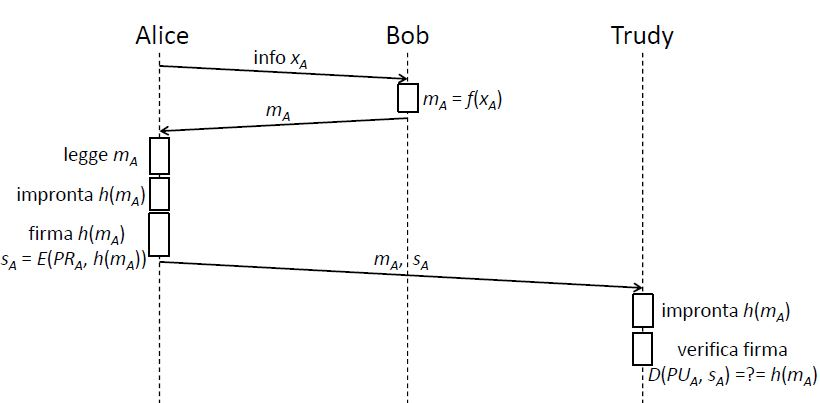
\includegraphics[height=10cm, width=10cm, keepaspectratio]{Immagini/hash/schema_hash_collisioni.JPG}}
	\caption{Scambio di messaggi nell'esempio\label{fig:esempio_res_coll}}
	\end{center}
\end{figure}
Se la funzione \textbf{non è resistente alla collisioni}, Bob potrebbe realizzare il seguente attacco:
\begin{enumerate}
\item calcola un messaggio $m'_{A} \mid h(m_{A}) = h(m'_{A})$
\item sottopone ad Alice $m_{A}$
\item quando Alice invia il messaggio a Trudy, Bob lo intercetta e sostituisce $m'_{A}$ a $m_{A}$
\item La verifica della firma di Trudy va a buon fine anche se l'autenticità è stata violata
\end{enumerate}
L'attacco è mostrato in \figurename~\ref{fig:esempio_res_coll_attack}.
\begin{figure}
	\begin{center}
	{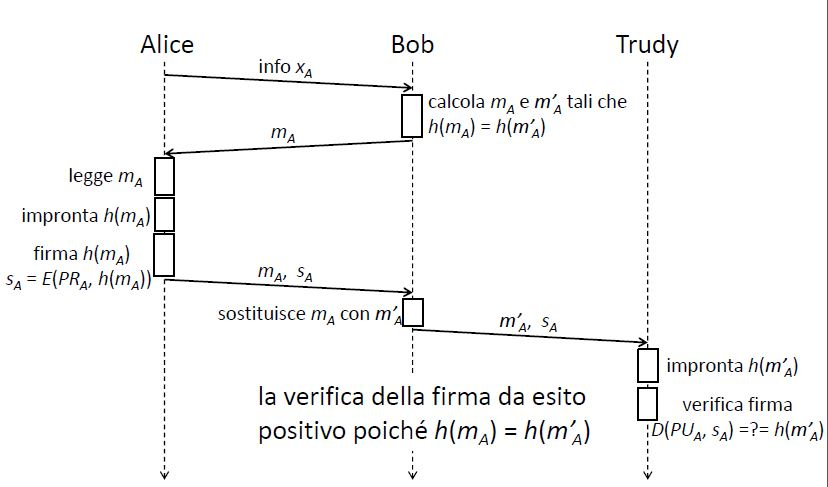
\includegraphics[height=10cm, width=10cm, keepaspectratio]{Immagini/hash/schema_hash_collisioni_1.JPG}}
	\caption{Attacco\label{fig:esempio_res_coll_attack}}
	\end{center}
\end{figure}

\subsubsection{Strategie di attacco - opzionale}
L'attacco, per come è presentato, sembra essere un attacco alla preimmagine (Bob deve calcolare un messaggio $m'_{A}$ avente un dato hash), non un attacco alle collisioni. Se si implementa seguendo questa filosofia, l'attacco è altamente inefficiente. Infatti, per calcolare $m'_{A}$, Bob deve:

\begin{enumerate}
\item dato $x_{A}$, calcolare prima il messaggio $m_{A}$ come desiderato da Alice;
\item genera un messaggio falsato $m'_{A}$;
\item esegue il test $h(m_{A}) == h(m'_{A})$;
\item in caso negativo ritornare al punto 2;
\end{enumerate}

In questo modo sono necessari circa $2^b$ tentativi (cioè $2^b$ messaggi falsati, poiché $\Pr \{h(m) = \hbar \} = \frac{1}{2^b}$) e non $2^{\frac{b}{2}}$. Il numero totale di messaggi generati può essere ridotto a $O(2^{\frac{b}{2}})$ sfruttando il paradosso del compleanno. Siano $L_m$ e $L_h$ due strutture dati dinamiche, ove memorizzare i messaggi e i relativi hash. A Bob conviene utilizzare il seguente algoritmo:
\begin{enumerate}
\item generare un messaggio $m_1$ che Alice firmerebbe;
\item calcolare l'hash $h_1 = h(m_1)$;
\item inserire $m_1$ in $L_m$ e $h_1$ in $L_h$ ;
\item posto $(i - 1) = \mid L_m \mid = \mid L_h \mid \: \text{con } i>1$, generare l'i-esimo messaggio $m_i$ nel seguente modo:
	\begin{itemize}
		\item se $i$ è pari, $m_i$ è un messaggio falsato secondo le intenzioni di Bob
		\item se $i$ è dispari, $m_i$ è un messaggio che Alice firmerebbe
	\end{itemize}
\item calcolare l'hash $h_i$ = $h(m_i)$;
\item verificare se $h_i \in L_h$;
	\begin{itemize}
		\item in caso negativo, inserire $m_i$ in $L_m$ e $h_i$ in $L_h$ e ritornare al punto 4
		\item in caso affermativo, recuperare il messaggio $m_j$ , con $j < i$, tale che $h_j = h_i$;
		\begin{itemize}
			\item se $m_i$ e $m_j$ hanno lo stesso significato (cioè se gli indici i e j sono entrambi pari o entrambi dispari), inserire $m_i$ in $L_m$ e $h_i$ in $L_h$ e ritornare al punto 4
			\item altrimenti ($m_i$ e $m_j$ sono due messaggi con significato diverso, ma con stesso hash) terminare la procedura e restituire la coppia $\langle m_i , m_j \rangle$
		\end{itemize}
	\end{itemize}
\end{enumerate}
Tale strategia permette di generare mediamente $O(2^{b/2})$ messaggi totali (contenuti cioè nelle strutture dati $L_m$ e $L_h$ per trovare una collisione. Si noti che:
\begin{equation} \label{eq:pr_coll_1}
\Pr \{ h(m_i) = h(m_j) \text{ AND } m_i \: e \: m_j  \mbox{ hanno significato diverso} \} \approx
\end{equation}
\begin{equation} \label{eq:pr_coll_2}
\approx \Pr \{m_i \: e \: m_j  \mbox{ hanno significato diverso} \} \cdot \Pr \{ h(m_i) = h(m_j) \} = 
\end{equation}
\begin{equation} \label{eq:pr_coll_3}
= \frac{1}{2} \cdot \Pr \{ h(m_i) = h(m_j) \}
\end{equation}
Per cui valgono (a meno di un fattore due moltiplicato per N) tutte le stime asintotiche di N (numero di messaggi generati) viste in precedenza. 
\newline \newline
Nell'approssimazione dalla \ref{eq:pr_coll_1} alla \ref{eq:pr_coll_2} si è tralasciata la dipendenza statistica tra il significato dei messaggi e l'output della funzione di hash. Tale contributo, se la funzione di hash è ben progettata (output pseudorandomico), è trascurabile. Nel passaggio dalla \ref{eq:pr_coll_2} alla \ref{eq:pr_coll_3} si è invece tenuto conto del fatto che mediamente nelle strutture dati sono contenuti per metà messaggi con il significato voluto da Bob e per metà con il significato voluto da Alice. 
\newline \newline
Sebbene il numero totale di messaggi generati sia asintoticamente pari a $O(2^{b/2})$, il tempo di esecuzione rimane $O(2^b)$ se non si utilizzano delle strutture dati ottimizzate per il confronto di stringhe. Infatti, la verifica effettuata nell'istruzione 6 richiede un tempo $O(\mid L_h \mid)$. Poiché tale istruzione viene effettuata per ogni inserimento, complessivamente, l'algoritmo richiede un tempo $O(\mid L_h \mid ^2)$. Poiché $\mid L_h \mid = O(2^{b/2})$, la complessità è $O(2^b)$. 
\newline \newline
Un tempo di esecuzione pari a $O(2^{b/2})$ è ottenibile utilizzando in luogo di una lista $L_h$ un \textbf{albero binario di ricerca}, un \textbf{tries} o un \textbf{suffix tree}. 

\section{Impieghi degli Algoritmi di Hash}
In combinazione con la \textbf{condivisione di un segreto}, l'algoritmo di hash può \textbf{sostituire} un algoritmo di crittografia a chiave segreta in ogni suo impiego (\textbf{Autenticazione a chiave segreta}, \textbf{Calcolo di MAC}, \textbf{Cifratura e Decifratura}).

\subsection{Autenticazione a chiave segreta}
Un possibile schema di autenticazione a chiave segreta (che segue il modello \textbf{sfida/risposta}) è mostrato in \figurename~\ref{fig:autenticazione_chiave_segreta_crit}, in cui:
\begin{itemize}
\item Alice invia un messaggio $r_A$ (la sfida) a Bob, e Bob si autentica, dimostrando di essere a conoscenza del segreto condiviso (la chiave $K_{AB}$) crittando il messaggio e restituendo il risultato (la risposta) ad Alice
\item Tramite il processo inverso Alice si autentica nei confronti di Bob.
\end{itemize}
\begin{figure}
	\begin{center}
	{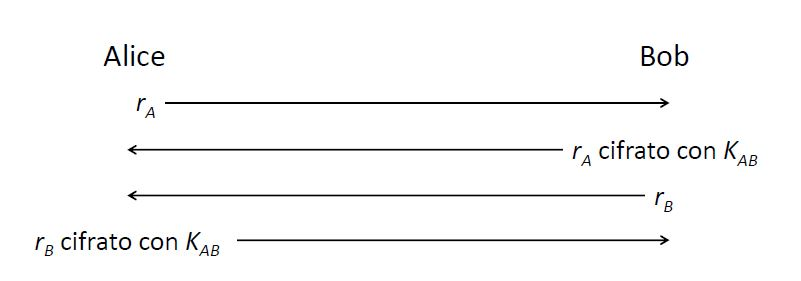
\includegraphics[height=8cm, width=8cm, keepaspectratio]{Immagini/hash/schema_autenticazione.JPG}}
	\caption{Mutua autenticazione tramite chiave segreta e crittografia simmetrica\label{fig:autenticazione_chiave_segreta_crit}}
	\end{center}
\end{figure}
Questo schema presenta delle vulnerabilità, che possono essere rimosse utilizzando alcuni accorgimenti, descritte nel paragrafo~\ref{par:aut_prot_mut_aut}. In ogni caso il protocollo può essere può essere implementato, anziché tramite la crittografia a chiave segreta, con una funzione di hash, come mostrato in \figurename~\ref{fig:autenticazione_chiave_segreta_hash}. Il meccanismo è lo stesso (e presenta le stesse vulnerabilità citate per lo schema precedente), ma la risposta consiste, invece che nella sfida crittografata, in un \textbf{message digest} calcolato tramite una funzione di hash che prende in input la concatenazione del messaggio e della chiave segreta.
\begin{figure}
	\begin{center}
	{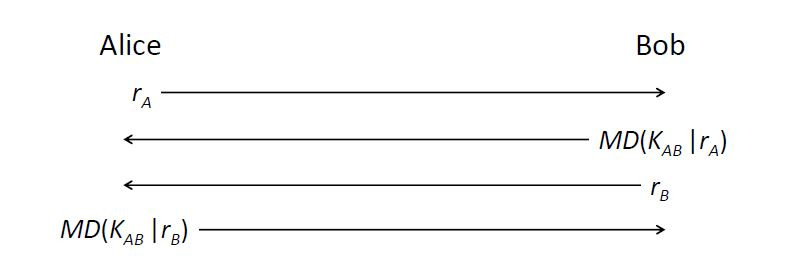
\includegraphics[height=8cm, width=8cm, keepaspectratio]{Immagini/hash/schema_autenticazione_md.JPG}}
	\caption{Mutua autenticazione tramite chiave segreta e funzione di hash \label{fig:autenticazione_chiave_segreta_hash}}
	\end{center}
\end{figure}

\subsection{Message Digest per MAC}
Un ulteriore possibile impiego delle funzioni di hash risiede nella generazione di codici MAC. Anche in questo caso è ovviamente necessario disporre di un segreto condiviso $K_{AB}$, poiché generare un MAC calcolandone semplicemente l'hash attraverso una data funzione non sarebbe sicuro. Infatti, se la funzione è pubblica, chiunque potrebbe calcolarlo. La soluzione più semplice è analoga a quella utilizzata nella mutua autenticazione: considerare $MD(K_{AB}\mid m)$ quale MAC di $m$. Tale soluzione è \textbf{teoricamente corretta}, ma presenta una debolezza derivante da una comune vulnerabilità dei principali algoritmi di digest (quali MD4, MD5, SHA-1). 

\subsubsection{Vulnerabilità di MD4, MD5, SHA-1}
\textbf{MD4}, \textbf{MD5} e \textbf{SHA-1} seguono il seguente schema generale:
\begin{enumerate}
\item dall'input $m$ si ottiene un messaggio $m_p$ avente lunghezza pari ad un multiplo intero di 512 bit. Ciò viene effettuato mediante un opportuno padding che include, tra l'altro, la lunghezza originaria di $m$
\item $m_p$ viene decomposto in chunk (pezzi) da 512 bit
\item il digest viene ottenuto mediante una procedura iterativa. Il digest all'n-esima iterazione dipende esclusivamente
\begin{itemize}
	\item dall'n-esimo chunk
	\item dal digest ottenuto all'(n – 1)-esima iterazione
\end{itemize}
\item il digest risultante di m è il digest ottenuto all'ultima iterazione
\end{enumerate}

Si assuma che un attaccante, Trudy, intercetti la coppia $\langle m, MD(K_{AB}|m) \rangle$ inviata da Alice a Bob. A questo punto Trudy, senza conoscere il segreto $K_{AB}$ (ma conoscendo l'algoritmo di digest), può calcolare il MAC di $\langle m^{*}, MD(K_{AB}|m^{*}) \rangle$, ove $m^{*}$ è un qualsiasi messaggio ottenuto concatenando $m_p$ con una qualsiasi stringa binaria, cioè:
\begin{equation}
m^{*} = m_p \mid s \quad \forall \: s \in \{0,1 \}^*
\end{equation}
Infatti la dipendenza dal segreto è stata già elaborata nei primi passi dell'algoritmo. Basta quindi "riprendere" l'algoritmo di digest dal primo chunk di $s$, utilizzando come digest al passo precedente il digest intercettato.
\newline \newline
Per mettere in sicurezza questa vulnerabilità sono state proposte diverse soluzioni. Esamineremo tali soluzioni, in ordine dalla più semplice alla più complessa (e che offre maggiori garanzie). 
\newline \newline
Una possibile soluzione è che il segreto $K_{AB}$ sia messo in coda. Tale soluzione è considerata sicura, a patto che l'algoritmo di digest sia \textbf{molto resistente alle collisioni}. Se così non fosse, ma fossero noti due messaggi $m_1$ e $m_2$ tali che $MD(m_1) = MD(m_2)$, per la vulnerabilità vista prima risulterebbe:
\begin{equation}
MD(m_1 \mid K) = MD(m_2 \mid K) \quad \forall K
\end{equation}
\newline
Un'altra possibilità è quella di utilizzare come MAC un sottoinsieme arbitrario del digest MD. Ad esempio, nel caso di digest a 128 bit, il MAC di $m$ può essere definito utilizzando i 64 bit meno significativi di $MD(K_{AB} \mid m)$. In questo modo un attaccante non può considerare il MAC come il digest ottenuto all'iterazione corrispondente al chunk che completa $m_p$, quindi non può calcolare il MAC di un qualunque messaggio
$m^{*}$ del tipo specificato senza conoscere $K_{AB}$. Precisamente l'attaccante, procedendo per tentativi, ha 1
chance su $2^{64}$ di ottenere l'altra metà di $MD(K_{AB}|m)$. Si osservi inoltre che considerare solo 64 bit
anziché i 128 del digest non comporta in pratica una perdita di sicurezza, poiché se l'attaccante non conosce $K_{AB}$ l'unica cosa che può fare è generare un MAC random a 64 bit e sperare che sia quello corretto.
\newline \newline 
Una terza soluzione è quella di inserire il segreto $K_{AB}$ sia in testa che in coda al messaggio m (il MAC è dato da $MD(K \mid m_1 \mid K)$). In questo modo $K_{AB}$ in testa fornisce resistenza alle collisioni e $K_{AB}$ in coda rende innocua la vulnerabilità insita negli algoritmi di hash.
\newline \newline
Infine un'ultima soluzione è rappresentata dall'algoritmo \textbf{HMAC} (keyed-Hash Message Authentication Code), che segue approssimativamente questo schema generale:
\begin{itemize}
\item concatena il segreto $K_{AB}$ in testa al messaggio
\item calcola il digest di tale combinazione
\item concatena il segreto $K_{AB}$ in testa a tale digest
\item calcola nuovamente il digest di quest'ultima combinazione
\end{itemize}
Si noti che HMAC applica due volte l'algoritmo di digest, rendendo il calcolo meno efficiente delle altre soluzioni. Tuttavia, il secondo digest può essere calcolato rapidamente: essendo costituito da un segreto concatenato ad un digest ha una lunghezza contenuta.

\subsection{Cifratura/Decifratura} 
Esploriamo ora la possibilità di utilizzare una funzione di hash come algoritmo di cifratura/decifratura. Poiché un hash ha una lunghezza fissa ed è non invertibile per definizione, devo trovare un modo per rendere invertibile la procedura. Una possibile soluzione è realizzare un cifrario a flusso, utilizzando un algoritmo MD per generare un keystream (flusso di bit pseudorandom dipendente dalla chiave). In altri termini, si può procedere in modo simile a quanto visto per la modalità operativa OFB (Output Feedback Mode) in \ref{par:ofb}. Devo utilizzare la funzione di hash potendo rendere tutto il processo invertibile, quindi introduco lo XOR tra un chunk del messaggio ed il \textbf{one time pad (OTP)} generato tramite funzione di hash (figura \ref{fig:otp}).
\begin{figure}
	\begin{center}
	{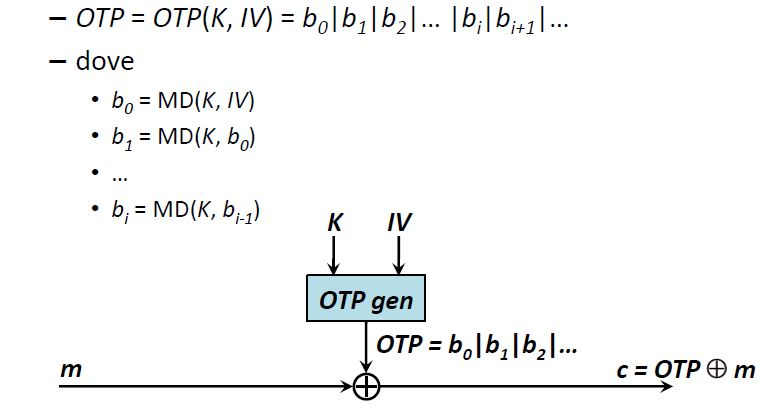
\includegraphics[height=10cm, width=10cm, keepaspectratio]{Immagini/hash/schema_cifratura_flusso.JPG}}
	\caption{Generazione OTP \label{fig:otp}}
	\end{center}
\end{figure}

\subsection{Hash tramite cifratura}
Si è visto che, in linea di principio, un algoritmo di digest può sostituire un algoritmo di cifratura/decifratura a chiave segreta in tutte le sue applicazioni. Naturalmente vale anche il viceversa, cioè, disponendo di un algoritmo di cifratura a chiave segreta, è possibile ottenere un algoritmo di digest.

\subsubsection{Esempio - UNIX Password Hash (Opzionale)}
Questo principio è utilizzato (ad esempio) per la gestione delle password in UNIX. UNIX non memorizza le password in chiaro, ma ne memorizza l'hash e, in fase di autenticazione, ricalcola l'hash della password ed esegue un confronto con il valore memorizzato. La generazione di hash per le password è illustrata in figura \ref{fig:pass_hash}.
\begin{figure}
	\begin{center}
	{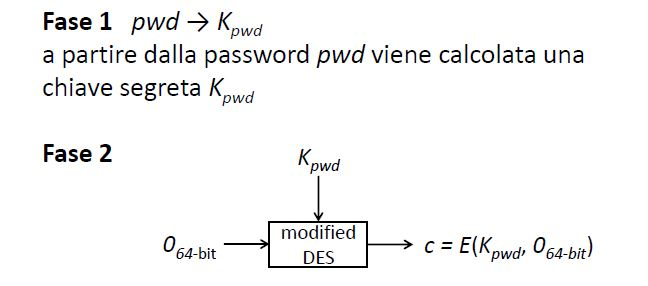
\includegraphics[height=8cm, width=8cm, keepaspectratio]{Immagini/hash/schema_des_come_hash.JPG}}
	\caption{Generazione hash di password in UNIX \label{fig:pass_hash}}
	\end{center}
\end{figure}
\begin{itemize}
\item Nella fase uno si determina una chiave segreta $K_{pwd}$ a partire dalla \textbf{password}
\item Nella fase due si ottiene h(pwd) come segue
\begin{enumerate}
	\item si considera una versione modificata di DES che dipende dal valore del \textbf{salt s} (numero di 12 bit generato in modo random, associato all'utente in esame). Il valore di s determina quali bit devono essere replicati nella fase di espansione di R da 32 a 48 bit
	\item l'algoritmo DES modificato è usato, con la chiave segreta K pwd , per cifrare la costante 0 (a 64 bit). UNIX memorizza per ciascun utente la stringa $s \mid h(pwd)$ nel file \textit{passwd}
\end{enumerate}
\end{itemize}
Ogni volta che una password \textbf{pwd} d'utente viene impostata viene generato il salt, \textbf{pwd} viene convertita in una chiave segreta $K_{pwd}$ a 64 bit, viene generato l'hash come descritto e il risultato e il salt vengono memorizzati nel file \textit{passwd}.
\newline \newline
Questo schema funziona bene, però, solamente per la cifratura di messaggi corti. Com'è possibile calcolare l'hash di un messaggio di lunghezza arbitraria utilizzando un algoritmo di cifratura a chiave segreta?
\subsection{Hash di grandi messaggi tramite algoritmi di cifratura}
Una possibile soluzione consiste nel suddividere il messaggio $m = m_{1},m_{2},m_{3},...,m_{n}$, e utilizzare ogni $m_{i}$ come input a un blocco in cascata. L'hash h(m) sarà l'output della cascata. Tale schema è mostrato in figura \ref{fig:hash_lung_ar}.
\begin{figure}
	\begin{center}
	{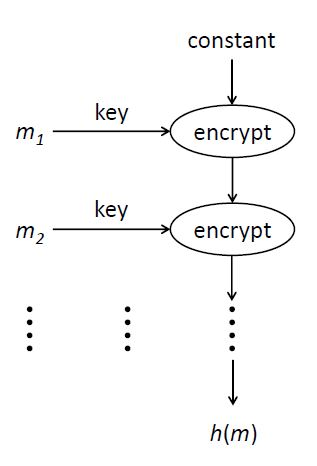
\includegraphics[height=5cm, width=5cm, keepaspectratio]{Immagini/hash/schema_des_come_hash_1.JPG}}
	\caption{Hash tramite cifratura per messaggi di lunghezza arbitraria \label{fig:hash_lung_ar}}
	\end{center}
\end{figure}
Tale schema ha però due debolezze:
\begin{enumerate}
\item Se si desidera individuare un messaggio $m$ avente un dato digest è possibile applicare un attacco simile a quello visto per DES doppio con chiavi distinte
\item $h(m)$ può risultare troppo corto. Infatti, in genere la lunghezza di un blocco è di 64 bit, e $2^{32}$ tentativi sono sufficienti per trovare due messaggi che collidono.
\end{enumerate}
Il primo problema è facilmente risolvibile rendendo l'output di ogni blocco differente diverso dall'input del successivo (ad esempio sommando (XOR) l'input e l'output di ciascun round, come mostrato in figura \ref{fig:hash_lung_ar_2}). 
\begin{figure}
	\begin{center}
	{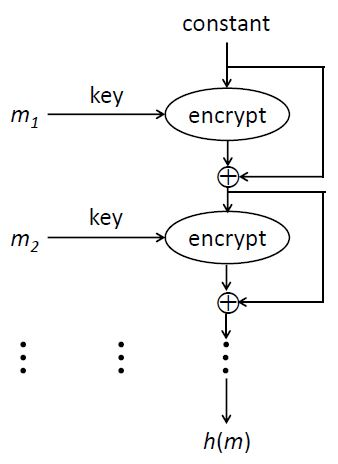
\includegraphics[height=5cm, width=5cm, keepaspectratio]{Immagini/hash/schema_des_come_hash_2.JPG}}
	\caption{Hash tramite cifratura per messaggi di lunghezza arbitraria con protezione\label{fig:hash_lung_ar_2}}
	\end{center}
\end{figure}
\newline \newline
Riguardo al problema 2, un hash di lunghezza doppia è facilmente ottenibile, calcolando un altro hash $h'(m)$ con la stessa tecnica - ma partendo da una costante diversa - e concatenandolo ad $h(m)$.